%Part of/Parte di https://github.com/f-dinucci/appuntiMeccanicaFluidi/
%License/Licenza Creative Commons Attribution-ShareAlike 4.0 International (CC BY-SA 4.0) - attribution/attribuzione Francesco Di Nucci
%See also/Vedere anche https://creativecommons.org/licenses/by-sa/4.0/ and/e https://creativecommons.org/licenses/by-sa/4.0/legalcode
%
\section{Legge dell'idrostatica}
%
\subsection{Legge dell'idrostatica}
Si affronterà ora il problema del calcolo della pressione nel caso statico (fluido fermo) con $\rho$ costante, che porterà alla legge dell'idrostatica.
Particolarizzando il bilancio di quantità di moto nel caso statico: 
	\begin{equation*}
		\begin{gathered}
			\cancel{\dv{t} \int{\uline{q} \dd{V}}} + \oint{\uuline{J}_Q \vdot \uline{n} \dd{S}} = \int{\uline{f} \dd{V}}\\
			0 + \oint{p \uline{n} \dd{S}} = \int{\rho \uline{g} \dd{V}}\\
			\text{usando la formula di Gauss}\\
			\int{p n_i \dd{S}} = \int{ \pdv{p}{x_i} \dd{V}}\\
			\text{che in notazione vettoriale equivale a} \\
			\oint{p \uline{n} \dd{S}} = \int{ \grad{p} \dd{V}} \\
			\text{quindi}\\
			\oint{p \uline{n} \dd{S}} = \int{\rho \uline{g} \dd{V}} \to \int_{V} {\grad{p} \dd{V}} = \int_{V} {\rho \uline{g} \dd{V}}
		\end{gathered}
	\end{equation*}
Questi sono integrali di volume su uno stesso volume $V$ qualsiasi, purché l'integrando sia una funzione continua\footnote{non è ovvio nella meccanica dei fluidi, ma in questo caso è tale} gli integrandi sono uguali:
	\begin{equation*}
		\grad{p} = \rho \uline{g}
	\end{equation*}
Si è arrivati ad una forma differenziale, facile da risolvere nel caso in cui $\rho$ sia una costante (evento piuttosto frequente):
	\begin{equation*}
		\begin{gathered}
			\grad{p} = \rho \uline{g} \quad \uline{g} = \left( 0, 0, -g \right) \quad \text{(preso z come asse verticale)}\\
			\text{quindi}\\
			\pdv{p}{x} = 0 \quad ; \quad \pdv{p}{y} = 0 \quad ; \quad \pdv{p}{z} = - \rho g\\
			p = - \rho g z + c \quad \textit{\textbf{Legge dell'idrostatica}}
		\end{gathered}
	\end{equation*}
Si ha quindi una espressione del campo\footnote{funzione esplicita delle coordinate e del tempo} di pressione. 
Questa può essere usata ad esempio per dimostrare il principio dei vasi comunicanti (ricordando che i peli liberi sono alla stessa pressione, atmosferica, dato che questa varia con differenze di quota di centinaia di metri)
Applicando la legge dell'idrostatica tra due quote di riferimento $z_0$ e $z$, e introducendo il peso specifico $\gamma = \rho g$, si ottiene:
	\begin{equation*}
		\begin{gathered}
			p = p_0 + \gamma (z_0 - z) \\
			\text{da cui si può ottenere} \\
			z + \frac{p}{\gamma} = cost. \quad \textbf{\textit{Legge di Stevino}}
		\end{gathered}
	\end{equation*}
%
\subsection{Vasi comunicanti}
%
	\begin{figure}[ht]
		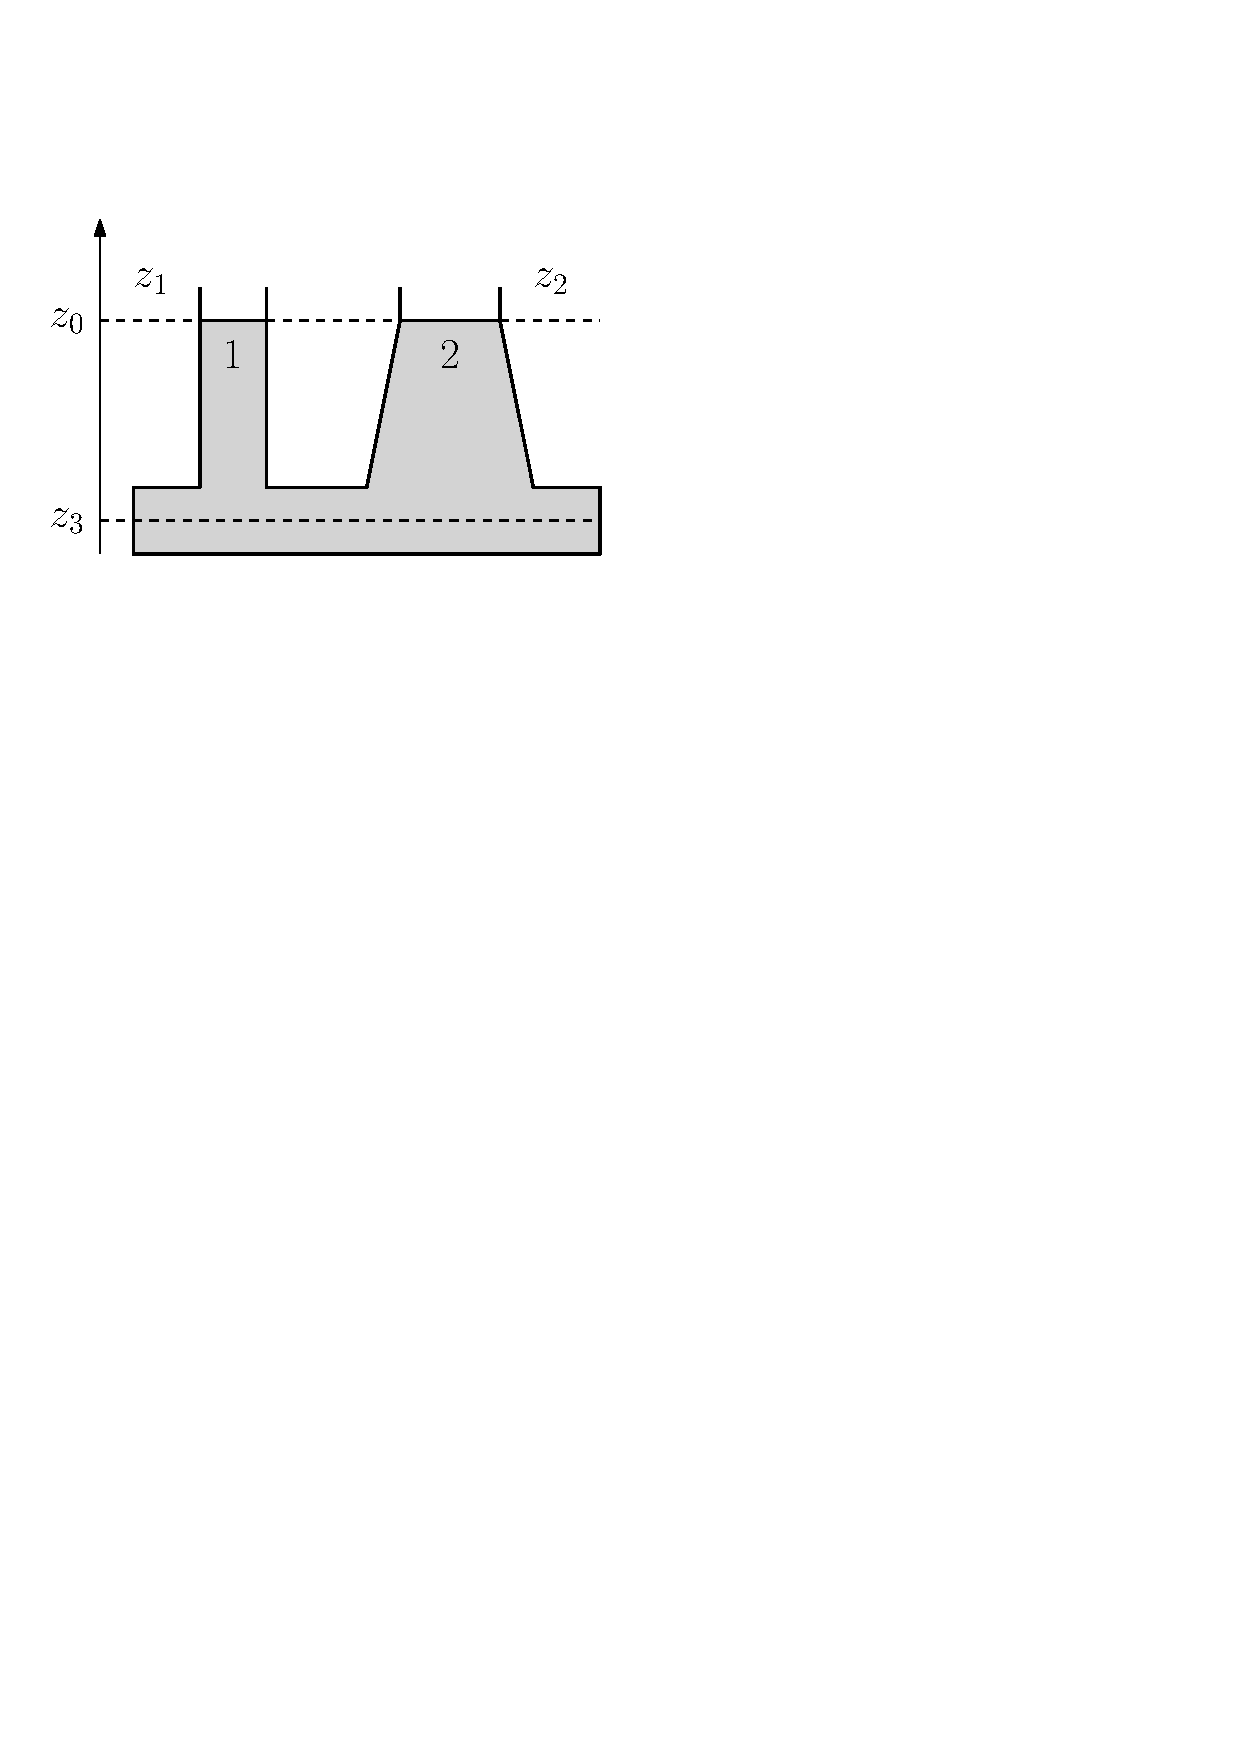
\includegraphics[scale=0.7]{./2.2 Legge dell'idrostatica/2.2-1}
		\centering
		\caption{Esempio di vasi comunicanti}
	\end{figure}
%
Secondo il principio dei vasi comunicanti, presi dei contenitori pieni di fluido e comunicanti tra loro tramite il fondo, all'equilibrio il pelo libero del fluido nei vari contenitori si troverà alla stessa altezza.
Questo vale sotto le ipotesi che nei vasi si trovi lo stesso fluido incomprimibile a riposo e che la geometria dei vasi sia tale da non generare fenomeni di capillarità\footnote{si può supporre che basti una sezione maggiore di $\SI{1}{\square \milli \metre}$}.
Il principio dei vasi comunicanti si può sia osservare empiricamente che dimostrare a partire dall'applicazione della legge dell'idrostatica tra due quote di riferimento (vedere \textit{Figura 2.2}):
	\begin{equation*}
		\begin{gathered}
			\text{applicando ai due contenitori la legge dell'idrostatica}\\
			p_3 = p_1 + \rho g (z_1 - z_3)\\
			p_3 = p_2 + \rho g (z_2 - z_3)\\
			\text{le due si possono uguagliare}\\
			p_1 + \rho g (z_1 - z_3) =   p_2 + \rho g (z_2 - z_3)\\
			\text{e dato che ambedue i peli liberi si trovano alla pressione atmosferica}\\
			\cancel{p_0} + \rho g (z_1 - z_3) =  \cancel{p_0} + \rho g (z_2 - z_3)\\
			\text{quindi} \quad z_1 = z_2
		\end{gathered} 
	\end{equation*}
Si è quindi dimostrato che i peli liberi del fluido nei vari contenitori si trovano alla stessa altezza. La stessa dimostrazione può essere ripetuta nel caso di \textit{n} contenitori diversi.
%
\subsection*{Bibliografia 2.2}
\cite[Cap.\ 3.1]{CengelCimbala}\\
\cite[Cap.\ 3.1]{PnueliGutfinger}